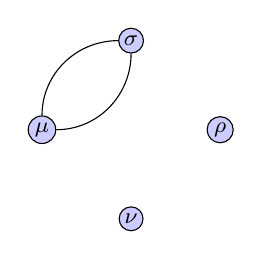
\begin{tikzpicture}[node distance=1.6cm]
\node (sigma) [draw, circle, inner sep=1pt, fill=blue!20, font=\bfseries] {\footnotesize $\sigma$};
\node (rho) [draw, circle, inner sep=1pt, fill=blue!20, font=\bfseries, below right of=sigma] {\footnotesize $\rho$};
\node (mu) [draw, circle, inner sep=1pt, fill=blue!20, font=\bfseries, below left of=sigma] {\footnotesize $\mu$};
\node (nu) [draw, circle, inner sep=1pt, fill=blue!20, font=\bfseries, below right of =mu] {\footnotesize $\nu$};
\draw (mu) to [out=90, in=180] (sigma);
\draw (sigma) to [out=-90, in=0] (mu);
\end{tikzpicture}
